%! Author = anton
%! Date = 28/08/2024

Starting with the previous performance, it may be interesting to analyse how performance changes as three main
parameters vary:
\begin{itemize}
    \item \(\tilde{\pi}\): represents prior probability of the positive class
    \item \(C_{fn}\): misclassification cost of a sample predicted as negative but it is positive
    \item \(C_{fp}\): misclassification cost of a sample predicted as positive but it is negative
\end{itemize}

\begin{table}[h]
    \centering
    \begin{tabular}{>{\centering\arraybackslash}p{2.9cm} >{\centering\arraybackslash}p{2.9cm} >{\centering\arraybackslash}p{2.9cm} >{\centering\arraybackslash}p{2.9cm}}
        \toprule
        & \textbf{MVG} & \textbf{Naive Bayes} & \textbf{Tied Covariance} \\
        \midrule
        \multicolumn{4}{c}{\textbf{Application \((\tilde{\pi},C_{fn}, C_{fp}) = (0.5, 1, 1)\)}} \\
        \midrule
        \textbf{actDCF} & 0.1399       & 0.1439               & 0.1860                   \\
        \textbf{minDCF} & 0.1302       & 0.1311               & 0.1812                   \\
        \midrule
        \multicolumn{4}{c}{\textbf{Application \((\tilde{\pi},C_{fn}, C_{fp}) = (0.9, 1, 1)\)}} \\
        \midrule
        \textbf{actDCF} & 0.4001       & 0.3893               & 0.4626                   \\
        \textbf{minDCF} & 0.3423       & 0.3509               & 0.4421                   \\
        \midrule
        \multicolumn{4}{c}{\textbf{Application \((\tilde{\pi},C_{fn}, C_{fp}) = (0.1, 1, 1)\)}} \\
        \midrule
        \textbf{actDCF} & 0.3051       & 0.3022               & 0.4061                   \\
        \textbf{minDCF} & 0.2629       & 0.2569               & 0.3628                   \\
        \midrule
        \multicolumn{4}{c}{\textbf{Application \((\tilde{\pi},C_{fn}, C_{fp}) = (0.5, 1, 9)\)}} \\
        \midrule
        \textbf{actDCF} & 0.3051       & 0.3022               & 0.4061                   \\
        \textbf{minDCF} & 0.2629       & 0.2569               & 0.3628                   \\
        \midrule
        \multicolumn{4}{c}{\textbf{Application \((\tilde{\pi},C_{fn}, C_{fp}) = (0.5, 9, 1)\)}} \\
        \midrule
        \textbf{actDCF} & 0.4001       & 0.3893               & 0.4626                   \\
        \textbf{minDCF} & 0.3423       & 0.3509               & 0.4421                   \\
        \bottomrule
    \end{tabular}
    \captionsetup{justification=justified,singlelinecheck=false,format=hang}
    \caption{Table showing minDCF and actDCF for different models and applications.}
    \label{tab:resultPerformanceClassifierWithoutPCA}
\end{table}

Analysing the results of the \autoref{tab:resultPerformanceClassifierWithoutPCA}, it is possible to observe:

\begin{table}[h]
    \centering
    \begin{tabular}{>{\centering\arraybackslash}p{2.9cm} >{\centering\arraybackslash}p{2.9cm} >{\centering\arraybackslash}p{2.9cm} >{\centering\arraybackslash}p{2.9cm}}
        \toprule
        & \textbf{MVG} & \textbf{Naive Bayes} & \textbf{Tied Covariance} \\
        \toprule
        \toprule
        \multicolumn{4}{c}{\textbf{Application \((\tilde{\pi},C_{fn}, C_{fp}) = (0.5, 1, 1)\)}} \\
        \midrule
        \multicolumn{4}{c}{\textbf{no PCA}} \\
        \midrule
        \textbf{actDCF} & 0.1399       & 0.1439               & 0.1860                   \\
        \textbf{minDCF} & 0.1302       & 0.1311               & 0.1812                   \\
        \midrule
        \multicolumn{4}{c}{\textbf{PCA}} \\
        \multicolumn{4}{c}{\textbf{\(m = 5\)}} \\
        \midrule
        \textbf{actDCF} & 0.1419       & 0.1749               & 0.1860                   \\
        \textbf{minDCF} & 0.1331       & 0.1737               & 0.1812                   \\
        \midrule
        \multicolumn{4}{c}{\textbf{\(m = 6\)}} \\
        \midrule
        \textbf{actDCF} & 0.1399       & 0.1780               & 0.1860                   \\
        \textbf{minDCF} & 0.1302       & 0.1727               & 0.1812                   \\
        \toprule
        \toprule
        \multicolumn{4}{c}{\textbf{Application \((\tilde{\pi},C_{fn}, C_{fp}) = (0.9, 1, 1)\)}} \\
        \midrule
        \multicolumn{4}{c}{\textbf{no PCA}} \\
        \midrule
        \textbf{actDCF} & 0.4001       & 0.3893               & 0.4626                   \\
        \textbf{minDCF} & 0.3423       & 0.3509               & 0.4421                   \\
        \midrule
        \multicolumn{4}{c}{\textbf{PCA}} \\
        \multicolumn{4}{c}{\textbf{\(m = 5\)}} \\
        \midrule
        \textbf{actDCF} & 0.3980       & 0.4660               & 0.4626                   \\
        \textbf{minDCF} & 0.3512       & 0.4340               & 0.4451                   \\
        \midrule
        \multicolumn{4}{c}{\textbf{\(m = 6\)}} \\
        \midrule
        \textbf{actDCF} & 0.4001       & 0.4512               & 0.4626                   \\
        \textbf{minDCF} & 0.3423       & 0.4359               & 0.4421                   \\
        \toprule
        \toprule
        \multicolumn{4}{c}{\textbf{Application \((\tilde{\pi},C_{fn}, C_{fp}) = (0.1, 1, 1)\)}} \\
        \midrule
        \multicolumn{4}{c}{\textbf{no PCA}} \\
        \midrule
        \textbf{actDCF} & 0.3051       & 0.3022               & 0.4061                   \\
        \textbf{minDCF} & 0.2629       & 0.2569               & 0.3628                   \\
        \midrule
        \multicolumn{4}{c}{\textbf{PCA}} \\
        \multicolumn{4}{c}{\textbf{\(m = 5\)}} \\
        \midrule
        \textbf{actDCF} & 0.3042       & 0.3930               & 0.4051                   \\
        \textbf{minDCF} & 0.2738       & 0.3545               & 0.3648                   \\
        \midrule
        \multicolumn{4}{c}{\textbf{\(m = 6\)}} \\
        \midrule
        \textbf{actDCF} & 0.3051       & 0.3920               & 0.4061                   \\
        \textbf{minDCF} & 0.2629       & 0.3535               & 0.3628                   \\
        \bottomrule
    \end{tabular}
    \captionsetup{justification=justified,singlelinecheck=false,format=hang}
    \caption{Show minDCF and actDCF for different models and applications before and after applying PCA.}
    \label{tab:resultPerformanceClassifierWithPCA}
\end{table}

\begin{figure}[h!]
    \centering
    \begin{subfigure}[b]{0.3\linewidth}
        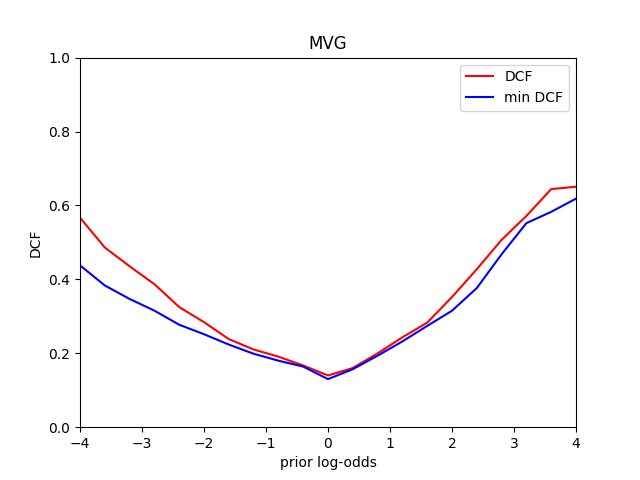
\includegraphics[width=\linewidth]{Lab/07. Lab 07/Images/01. MVG}
        \caption{MVG}
        \label{fig:dcfMVG}
    \end{subfigure}
    \begin{subfigure}[b]{0.3\linewidth}
        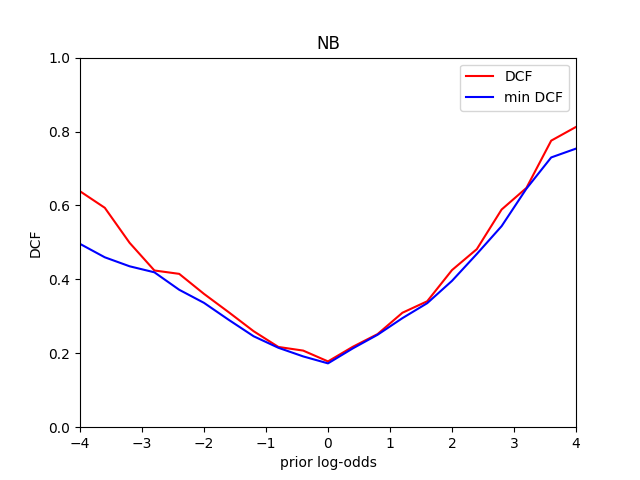
\includegraphics[width=\linewidth]{Lab/07. Lab 07/Images/02. Naive Bayes}
        \caption{Naive Bayes}
        \label{fig:dcfNB}
    \end{subfigure}
    \begin{subfigure}[b]{0.3\linewidth}
        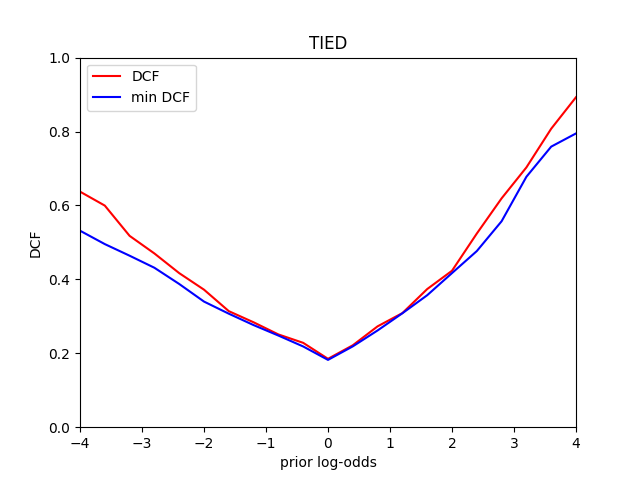
\includegraphics[width=\linewidth]{Lab/07. Lab 07/Images/03. Tied}
        \caption{Tied Covariance}
        \label{fig:dcfTC}
    \end{subfigure}
    \caption{Error Bayes plots}
    \label{fig:dcfMVGNBTC}
\end{figure}